\documentclass[11pt]{article}

\textwidth 16cm \textheight 23cm \evensidemargin 0cm
\oddsidemargin 0cm \topmargin -2cm
\parindent 0pt
\parskip \medskipamount


\usepackage[dutch]{babel}
\usepackage{amssymb}
\usepackage{amsmath}
\usepackage[utf8]{inputenc}
\usepackage[normalem]{ulem} % strikethrough normal text with \sout{text}
\usepackage{cancel} % strikethrough in math mode with \cancel{text}
\usepackage{hyperref}

\usepackage{subfig}
\usepackage{wrapfig}
\usepackage{graphicx}

\usepackage[table]{xcolor}

\usepackage{pgf,tikz}
\usetikzlibrary{arrows}

\usepackage{color}
\newcommand{\todo}[1]{\textcolor{red}{\##1\#}}
\newcommand{\question}[1]{\textcolor{blue}{\##1\#}}

\newcommand{\vraag}[2]{\begin{itemize}\item {\it #1} \vspace{#2}\end{itemize}}

\newcommand{\degree}{\ensuremath{^\circ}}

\graphicspath{{../figuren/}}

\begin{document}

\section{Iets statistisch onderzoeken}

We wensen een statistisch onderzoek uit te voeren. Wat wil dit nu zeggen? Wel, {\it onderzoeken} is iets nauwkeurig nazien of nagaan. Een voorbeeld zou kunnen zijn: {\it Tot hoe laat mogen jongeren in het weekend uitgaan?}. De vraag die bij een onderzoek hoort noemen we de {\bf onderzoeksvraag}. Een {\it statistisch onderzoek} is dan een onderzoek die verloopt volgens de statistiek. De {\bf statistiek} is de wetenschap van het waarnemen van verschijnselen en het weergeven van de uitkomsten in getallen en figuren. In het vorig voorbeeld wil dit zeggen dat we {\it waarnemen} bij anderen tot hoe laat deze uitgaan. Deze waarnemingen gaan we dan zo goed mogelijk {\it weergeven}, dit met getallen of figuren.

Een onderzoek kan in vier stappen verlopen:
\begin{enumerate}
  \item Wat wil je weten? Hoe ga je meten?
  \item Op speurtocht gaan in de dataset.
  \item Wat heb je gevonden? Hoe ver kan je gaan in je conclusie?
  \item Kernachtig samenvatten van onderzoek.
\end{enumerate}

Wat de stappen inhouden zullen we zien aan de hand van een aantal voorbeelden.

\section{Statistisch onderzoek naar de kleuren van M\&M-snoepjes}

\subsection{De onderzoeksvraag}

\begin{wrapfigure}{r}{0.4\textwidth}
  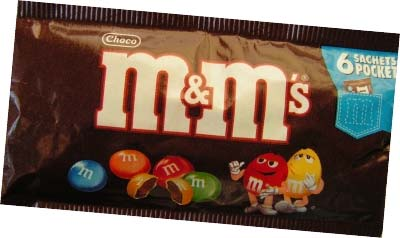
\includegraphics[width=0.4\textwidth]{MenM-verpakking.png}
\end{wrapfigure}

Iedereen kent wel M\&M’s, de chocoladesnoepjes met de felgekleurde suikerjasjes. De fabrikant van
M\&M’s stopt verschillende kleuren snoepjes in één verpakking.

Heb je enig idee welke kleuren allemaal voorkomen bij M\&M’s?
Komt elke kleur evenveel voor? Dat ga je nu onderzoeken.

Je hebt hier al een eerste probleem. Wat wil je eigenlijk
onderzoeken? Wil je iets zeggen over de kleuren in je eigen zakje
M\&M”s of wil je iets zeggen over de kleuren van alle M\&M-
snoepjes die door de fabrikant gemaakt worden? Dat zijn nogal
verschillende vragen!

\subsection{Wat wil je weten? Hoe ga je meten?}

\subsubsection{Een dataset maken}

Om goed het onderscheid te maken tussen “alle M\&M’s” en “de snoepjes in jouw zakje M\&M’s”
gebruikt de statistiek twee verschillende woorden. Je spreekt over {\bf populatie} als je “de totale
verzameling” bedoelt (dus alle M\&M-snoepjes). Meestal heb je geen tijd of geld om een volledige
populatie te onderzoeken en daarom bekijk je enkel een klein deeltje van die populatie. Zo’n deeltje
van een populatie wordt in de statistiek een {\bf steekproef} genoemd. De snoepjes die in je zakje
M\&M’s zitten, zijn een heel klein deeltje van alle M\&M’s. Jouw snoepjes zijn dus een steekproef uit
de totale populatie van alle M\&M’s.

Je steekproef bestaat uit dingen die je zelf hebt verzameld, die je dus zelf kan zien en beschrijven
(met getallen en grafieken). Hoe je dat doet, dat ga je in dit onderzoek leren. Maar misschien wil je
daarna ook iets zeggen over alle M\&M’s. Misschien zijn de blauwe snoepjes in jouw zakje in de
meerderheid. Zou je dan kunnen zeggen dat bij alle M\&M’s de blauwe snoepjes het meest
voorkomen? (Let op! Misschien heeft een andere leerling meer rode snoepjes).

Iets zeggen over de totale populatie als je enkel de steekproef ziet, dat is helemaal niet eenvoudig.
Statistiek kan je hierbij helpen. Een eerste hulp die de statistiek je biedt, gaat over de manier waarop
je een steekproef moet trekken. De raadgeving die je hier krijgt, had je waarschijnlijk nooit
verwacht. Om een goede steekproef te trekken, moet je je laten leiden door ... het toeval!

Je laten leiden door het toeval, dat is gemakkelijker gezegd dan gedaan. M\&M's worden gemaakt in verschillende
kleuren volgens een verhouding die door de fabrikant is vastgelegd. Die snoepjes komen terecht in
een reuzegrote container waar ze grondig door elkaar worden gemengd. Daarna wordt uit die
container lukraak een schep snoepjes genomen en die snoepjes worden in een zakje verpakt. Dat
gebeurt natuurlijk allemaal volautomatisch en in superhygiënische omstandigheden.

Die enorme container, waarin miljoenen M\&M’s zitten, kan je beschouwen als een goed model voor
de hele populatie. Een goede steekproef trek je dan als volgt: “goed mengen en dan lukraak trekken”.
Deze manier van werken krijgt in de statistiek de naam “{\bf enkelvoudige aselecte steekproef}”. Het
aantal elementen in je steekproef (het aantal getrokken snoepjes) noteer je door de letter “$n$” (dat
noem je de {\bf steekproefgrootte}).

De informatie in je steekproef ga je nu op een overzichtelijke manier opschrijven in een tabel. Zo krijg je de
{\bf gegevensverzameling of dataset}. In zulk een tabel staan op de rijen de {\bf elementen}, deze zijn de objecten die in een statistische studie worden onderzocht. In ons geval heb je voor elke M\&M één rij. In de kolommen staan de {\bf veranderlijken}, elke veranderlijke is één welbepaalde eigenschap die je opmeet. Zo kunnen we voor elke M\&M de kleur noteren.

\vraag{Maak een tabel waarin je de gegevens zal opschrijven. Als je afkortingen gebruikt, schrijf dan ook op wat die afkortingen betekenen.}{10cm}

\subsubsection{De dataset: getallen en context}
Bij de dataset die je pas hebt opgesteld is er één kolom waarin je de kleur van de snoepjes hebt
geschreven. Je hebt hier te maken met een “eigenschap van snoepjes”, namelijk “hun kleur”. Dit is
een “veranderlijke” die jij hebt opgemeten. Deze veranderlijke heeft hier de waarden: rood, groen,
blauw, bruin, en geel.
Op kleuren kan je geen zinvolle wiskundige bewerkingen uitvoeren zoals optellen of
vermenigvuldigen. Daarom noemt men de veranderlijke “kleur” een {\bf kwalitatieve veranderlijke}.

Er is een belangrijk onderscheid tussen de naam van een veranderlijke en de
verschillende waarden van die veranderlijke.
In dit geval is “kleur” de {\bf naam} van de veranderlijke en “rood, groen, blauw,
...” zijn de mogelijke {\bf waarden}.

\subsection{Op speurtocht in de dataset}

Je dataset is de basis voor al je verder onderzoek. De dataset, samen met de beschrijving van hoe je
hem hebt opgemeten, moet je nauwkeurig bewaren.

\subsubsection{Een frequentietabel opstellen}

\vraag{Gebruik je dataset om een frequentietabel op te stellen. Doe dat zoals hieronder aangegeven.}{0cm}

In de eerste kolom schrijf je de kleuren en in de tweede kolom schrijf je hoeveel snoepjes er van die
kleur zijn. Dit aantal heet de {\bf frequentie} van die kleur. Een tabel die je op deze manier opstelt, heet
een {\bf frequentietabel}. Zorg ervoor dat je elke kolom een juiste naam geeft: deze naam schrijf je
bovenaan de kolom.

\begin{center}
  \begin{tabular}{|p{2cm}|p{2cm}|p{2cm}|}
    \hline
    &&\vspace*{0pt}\\
    \hline
    &&\vspace*{0pt}\\
    \hline
    &&\vspace*{0pt}\\
    \hline
    &&\vspace*{0pt}\\
    \hline
    &&\vspace*{0pt}\\
    \hline
    &&\vspace*{0pt}\\
    \hline
    &&\vspace*{0pt}\\
    \hline
  \end{tabular}
\end{center}
\vspace{1cm}

\vraag{Hoe kan je de steekproefgrootte snel berekenen met behulp van de frequentietabel?}{4cm}

We gaan nu een derde kolom aan de frequentietabel toevoegen. In die kolom komt, per kleur, {\bf de
relatieve frequentie}. De relatieve frequentie is niets anders dan de frequentie gedeeld door het totale
aantal $n$ . Je kan dit getal ook in percent uitdrukken. Als je voor “geel” een relatieve frequentie van
0.16 vindt, dan kan je dat ook schrijven als 16\%. Hierbij rond je af op één eenheid. In woorden zeg
je dat 16\% van jouw onderzochte snoepjes geel is.

Om zoveel mogelijk van je tijd te kunnen besteden aan nadenken en
discussiëren, ga je zo weinig mogelijk tijd besteden aan slaafse
berekeningen. We gebruiken software op een verstandige manier. Zo leer je ook
hoe elk “echt” statistisch onderzoek verloopt.

We starten {\it Geogebra} en kiezen 'Beeld-Rekenblad' om het rekenblad te tonen. Het algebravenster en het tekenblad mogen verborgen worden. De eerste kolom vullen we met de frequenties. Als je bijvoorbeeld $13$ rode, $9$ groene, $8$ gele, $7$ oranje, $7$ bruine en $6$ blauwe snoepjes had, dan ga je als volgt te werk. In de eerste {\bf cell} rechtsboven vul je 13 in. Deze cell noemt A1. In de cell eronder vul je $9$ in. Je gaat zo verder tot aan cell A6. De cellen A1 tot aan A6 noteren we met A1:A6 en deze wordt een {\bf lijst} genoemd.

In de tweede kolom, in cell B1, vul je \verb#=A1 / Som[$A$1:A6]# in. Het gelijk aan teken '=' maakt aan Geogebra duidelijk dat wat volgt berekend moet worden. Geogebra zal in dit geval de waarde in de cell A1 delen door de som van de cellen in de lijst A1:A6. Nu doen we dit ook voor de andere cellen in de tweede kolom, waarbij dan op de juiste plaats A1 vervangen wordt.

\begin{center}
  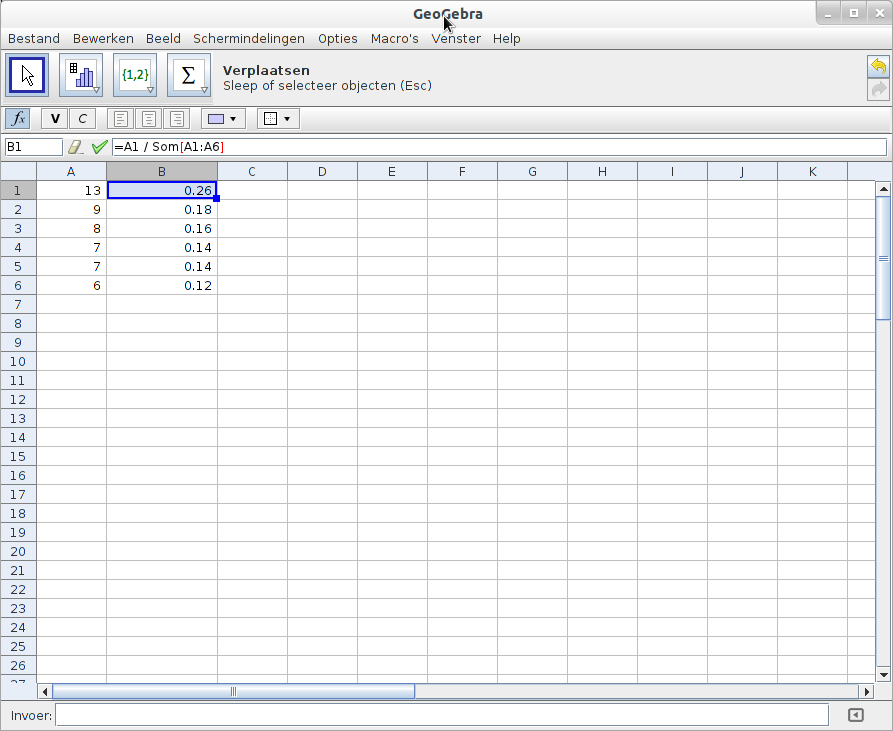
\includegraphics[width=14cm]{gg-relatieve_frequentie.png}
\end{center}

\vraag{Voeg aan je tabel een derde kolom toe met naam “relatieve frequentie” en schrijf daarin de
resultaten die in Geogebra staan (in percent). Tel de percenten bij elkaar op. Hoeveel heb je?
}{3cm}

Soms heb je frequenties nodig, in andere gevallen gebruik je relatieve frequenties. Als je aantallen
bestudeert, dan werk je met frequenties. Als je percentages gebruikt om twee onderzoeken met
elkaar te vergelijken, dan werk je met relatieve frequenties.

{\bf Voorbeeld}\\
Om te weten of je genoeg rode snoepjes hebt om er eentje te kunnen geven aan elk van je 10
vrienden, dan kijk je naar de frequentie.
Als je de kleurensamenstelling van een grote en een kleine zak M\&M’s wil vergelijken, dan zal je
met percentages werken en dus relatieve frequenties gebruiken.



\subsubsection{Figuren tekenen}

\begin{wrapfigure}{r}{0.3\textwidth}
  \vspace{-0.5cm}
  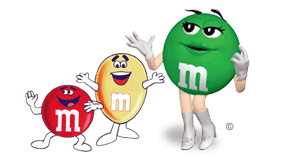
\includegraphics[width=0.3\textwidth]{MenM-fun.png}
\end{wrapfigure}

Veruit het meest belangrijke onderdeel bij de studie van een
dataset is kijken naar figuren. Dit is niet eenvoudig en je
moet stapsgewijs leren waar je allemaal moet op letten.
Zodra je dit wat kent, kan je uit een figuur heel veel
informatie halen. Maar je moet natuurlijk eerst weten welke
figuur je moet maken en hoe je die moet tekenen.

\subsubsection*{Een staafdiagram}

Je hebt in dit onderzoek een nominaal kwalitatieve veranderlijke opgemeten. Voor dit soort
veranderlijken is het {\bf staafdiagram} de basisfiguur.

Als voorbeeld zie je hier een staafdiagram
van de Vlaamse bevolking per provincie. De
informatie die hier wordt weergegeven, kan
je vinden in het boekje “Vlaanderen in
cijfers” op de website:
\url{http://www4.vlaanderen.be/dar/svr/Cijfers/Pages/Excel.aspx}.

De namen van de provincies zijn afgekort als:
  
\begin{minipage}{0.5\textwidth}
  \begin{description}
    \item[Antw] Antwerpen,
    \item[O-Vl] Oost-Vlaanderen,
    \item[W-Vl] West-Vlaanderen,
    \item[Vl-Br] Vlaams - Brabant,
    \item[Limb] Limburg.
  \end{description}
\end{minipage}
\begin{minipage}{0.5\textwidth}
%  \definecolor{qqqqff}{rgb}{0,0,1}
\begin{tikzpicture}[scale=0.1,line cap=round,line join=round,>=triangle 45,x=1.0cm,y=1.0cm]
\draw[-,color=black] (-9.63,0) -- (78.66,0);
\draw[color=black] (60,0.13) node [anchor=south west] { Provincie};
\draw[-,color=black] (0,-4.46) -- (0,27.9);
\draw[color=black] (0.57,27.25) node [anchor=west] { Aantal inwoners};
\clip(-9.63,-4.46) rectangle (78.66,27.9);
\draw[fill=black,fill opacity=0.1] (7,0) rectangle (12.5,8.39);
\draw[fill=black,fill opacity=0.1] (12.5,0) rectangle (17.5,0);
\draw[fill=black,fill opacity=0.1] (17.5,0) rectangle (22.5,10.77);
\draw[fill=black,fill opacity=0.1] (22.5,0) rectangle (27.5,0);
\draw[fill=black,fill opacity=0.1] (27.5,0) rectangle (32.5,11.59);
\draw[fill=black,fill opacity=0.1] (32.5,0) rectangle (37.5,0);
\draw[fill=black,fill opacity=0.1] (37.5,0) rectangle (42.5,14.32);
\draw[fill=black,fill opacity=0.1] (42.5,0) rectangle (47.5,0);
\draw[fill=black,fill opacity=0.1] (47.5,0) rectangle (52.5,17.45);
\draw (48.1,-0.39) node[anchor=north west] {Antw};
\draw (18.33,-0.43) node[anchor=north west] {Vl-Br};
\draw (28.4,-0.43) node[anchor=north west] {W-Vl};
\draw (38.13,-0.43) node[anchor=north west] {O-Vl};
\draw (7.91,-0.36) node[anchor=north west] {Limb};
\draw (46.85,24) node[anchor=north west] {1744862};
\draw (16.74,18) node[anchor=north west] {1076924};
\draw (26.93,12.35) node[anchor=north west] {1159366};
\draw (36.66,15.08) node[anchor=north west] {1432326};
\draw (7.23,9.13) node[anchor=north west] {838505};
\begin{scriptsize}
\fill [color=qqqqff] (0,0) circle (1.5pt);
\end{scriptsize}
\end{tikzpicture}

  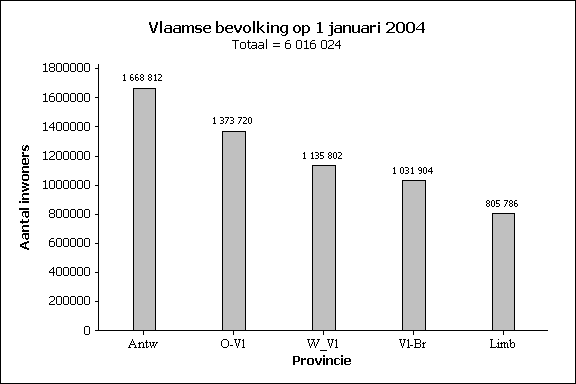
\includegraphics[width=0.5\textwidth]{vlaamse_bevolking.png}
\end{minipage}

Om een staafdiagram te tekenen op basis van jouw frequentietabel ga je als volgt te werk:
\begin{enumerate}
  \item Op de x-as zet je de verschillende kleuren. Hoewel de waarden van een nominale
veranderlijke geen natuurlijke volgorde hebben, zal je toch moeten kiezen hoe je de kleur
ordent op de x-as. Welke kleur komt als eerste? Welke kleur komt als tweede? Waarom maak
je die keuze?

De kleuren van een snoepje hebben geen natuurlijke volgorde. We rangschikken daarom de
bijhorende frequenties. Dat zijn getallen en die hebben wel een natuurlijke volgorde. Je kan
bijvoorbeeld rangschikken van groot naar klein. Voor kleuren met gelijke frequenties kan je
de onderlinge plaats zelf kiezen.
\item Op de y-as duid je de frequentie van elke kleur aan en je tekent dan bij elke kleur een staafje
waarvan de lengte overeenkomt met de frequentie van die kleur. Zorg ervoor dat alle staafjes
los van elkaar staan.
\item Voorzie de assen van de juiste naam.
\end{enumerate}

\vraag{Teken nu zo’n staafdiagram voor jouw onderzoek.}{0cm}
\begin{center}
\definecolor{qqqqff}{rgb}{0,0,1}
\begin{tikzpicture}[line cap=round,line join=round,>=triangle 45,x=1.0cm,y=1.0cm]
\draw[-,color=black] (0,0) -- (10,0);
\draw[-,color=black] (0,0) -- (0,10);
\end{tikzpicture}

\end{center}

Zulk staafdiagram kan ook met Geogebra gemaakt worden:
\begin{enumerate}
  \item Vul een rekenblad in met de frequenties.
  \item Maak vanuit het rekenblad een lijst aan van de frequenties aan door B2:B7 te selecteren, rechts te klikken en creëer lijst te kiezen. Hernoem de nieuw aangemaakte lijst met naam "lijst 1', door deze te selecteren in het algebra venster en met het toetsenbord "frequentie" te typen.
  \item Maak ook een lijst met posities aan. Typ hiervoor in het invoervenster\\
  \verb$posities={10,20,30,40,50,60,70}$.
  \item Teken nu het staafdiagram met het commando \verb$Staafdiagram[posities,frequenties,5]$
  \item Wijzig nu de schaal van de assen door deze te verslepen.
  \item Voeg nu tekst in om alle labels aan te vullen.
\end{enumerate}

\begin{center}
  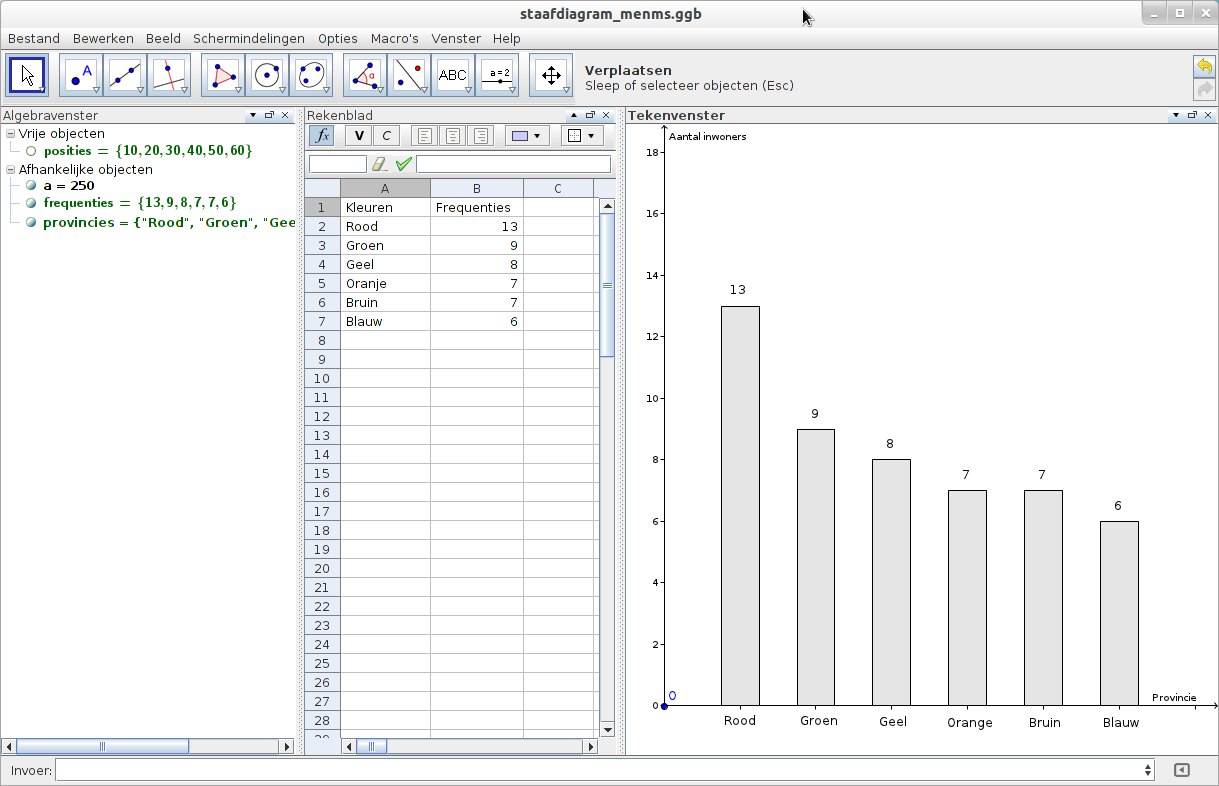
\includegraphics[width=14cm]{gg-staafdiagram_menms}
\end{center}

\subsubsection*{Een taartdiagram}
Misschien wil je de relatieve frequenties van de kleuren grafisch voorstellen. Dan kan je ook een
staafdiagram tekenen, waarbij je in de y-richting staafjes tekent waarvan de lengte gelijk is aan de
relatieve frequentie.
Maar er is ook een andere figuur die de relatieve frequentie (meestal uitgedrukt in percent) mooi
weergeeft. Dat is het {\bf taartdiagram of cirkeldiagram}.

Bij het tekenen van een taartdiagram verdeel je een cirkeloppervlak in stukken, juist zoals je een
taart in stukken snijdt. Zo’n stuk heet een {\bf sector}. De totale oppervlakte van de cirkel komt overeen
met de som van alle percentages en dat is 100\%.

\begin{wrapfigure}[13]{r}{0.3\textwidth}
  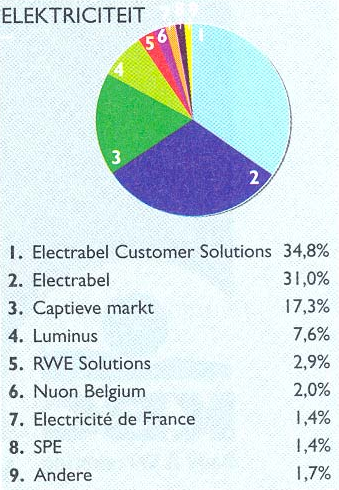
\includegraphics[width=0.3\textwidth]{cirkeldiagram_electriciteit}
\end{wrapfigure}

Voor een taartdiagram maken we enkele afspraken:
\begin{itemize}
  \item Begin bovenaan en draai naar rechts.
  \item De grootste sector komt eerst, dan komt de tweede
grootste, enzovoort.
\end{itemize}

Je ziet hier een voorbeeld van de marktaandelen van
energiebevoorraders in België. Het gaat over de elektriciteit in
het jaar 2004. Deze figuur staat in het weekblad Knack van 22
juni 2005 en is goed leesbaar. Maar als je een krant of
weekblad doorbladert, dan zie je soms verwarrende en zelfs
verkeerde grafieken.

Hoeveel graden elke sector is, bereken je door de relatieve
frequentie te vermenigvuldigen met $360\degree$. Dit doe je met je
rekenmachine. Maak daarna “verstandige” afrondingen zodat
alle sectoren samen terug $360\degree$ geven (je kan
eventueel enkele keren tot op een halve graad werken).

Om een taartdiagram te tekenen op basis van jouw onderzoek begin je als volgt.
\vraag{Bereken eerst voor elke relatieve frequentie hoe groot de sector is die daarbij hoort. Gebruik
je rekenmachine.}{0cm}

\begin{center}
  \begin{tabular}{|p{1.5cm}|p{1.5cm}|p{1.5cm}|p{1.5cm}|p{1.5cm}|p{1.5cm}|p{1.5cm}|}
    \hline
    kleur:\vspace{0.5cm}&&&&&&\\
    \hline
    hoek:\vspace{0.5cm}&&&&&&\\
    \hline
  \end{tabular}
\end{center}

\vraag{Teken nu cirkelsectoren die overeenstemmen met de relatieve frequenties. Schrijf bij elke
sector met welke kleur van snoepje hij overeenkomt en noteer ook de relatieve frequentie in
percentvorm erbij. Je kan natuurlijk ook de sector inkleuren met de bijhorende kleur.}{2cm}

\begin{center}
  \begin{tikzpicture}[line cap=round,line join=round,>=triangle 45,x=1.0cm,y=1.0cm]
\clip(0,0) rectangle (10,10);
\draw(5,5) circle (5cm);
\draw (5,5)-- (5,10);
\end{tikzpicture}

\end{center}

Ook met Geogebra kunnen we een cirkeldiagram maken. We vertrekken vanuit het zelfde bestand als bij
het staafdiagram. De frequentie moeten we nu omzetten naar het aantal graden dat het sector is. Maak
hiervoor eerst het totaal van alle frequenties door in cell B9 \verb$=Som[B2:B7]$ als formule te nemen.
Vul nu in de cel C2, naast de frequentie, het volgende als formule in: \verb#=B2 / $B$9 * 360#$\degree$.
Je kan nu de cell rechts-onder vastnemen en verslepen, Geogebra vult nu automatisch de juiste cellnamen in.

Nu we de graden hebben berekend voor de sectoren van het cirkeldiagram maken we de figuur. Creëer eerst twee punten. $A$ op $(0,0)$ en $B$ op $(0,5)$. Creëer nu een cirkel met als middelpunt $A$ en als straal $B$. Klik nu op het icoontje {\it Hoek met gegeven grootte}. Klik eerst op $B$ en dan op $A$ en als hoekgrootte geef je \verb$C2$ in. Klik nu op het icoontje {\it Cirkelsector met middelpunt door 2 punten}. Als eerste punt geef je $A$, als tweede punt geef je $B'$ en uiteindelijk als derde punt geef je $B$. Herhaal dit nu voor de andere sectoren.

De figuur kan afgewerkt worden door tekst in te voeren en de kleuren van de sectoren te wijzigen:
\begin{center}
  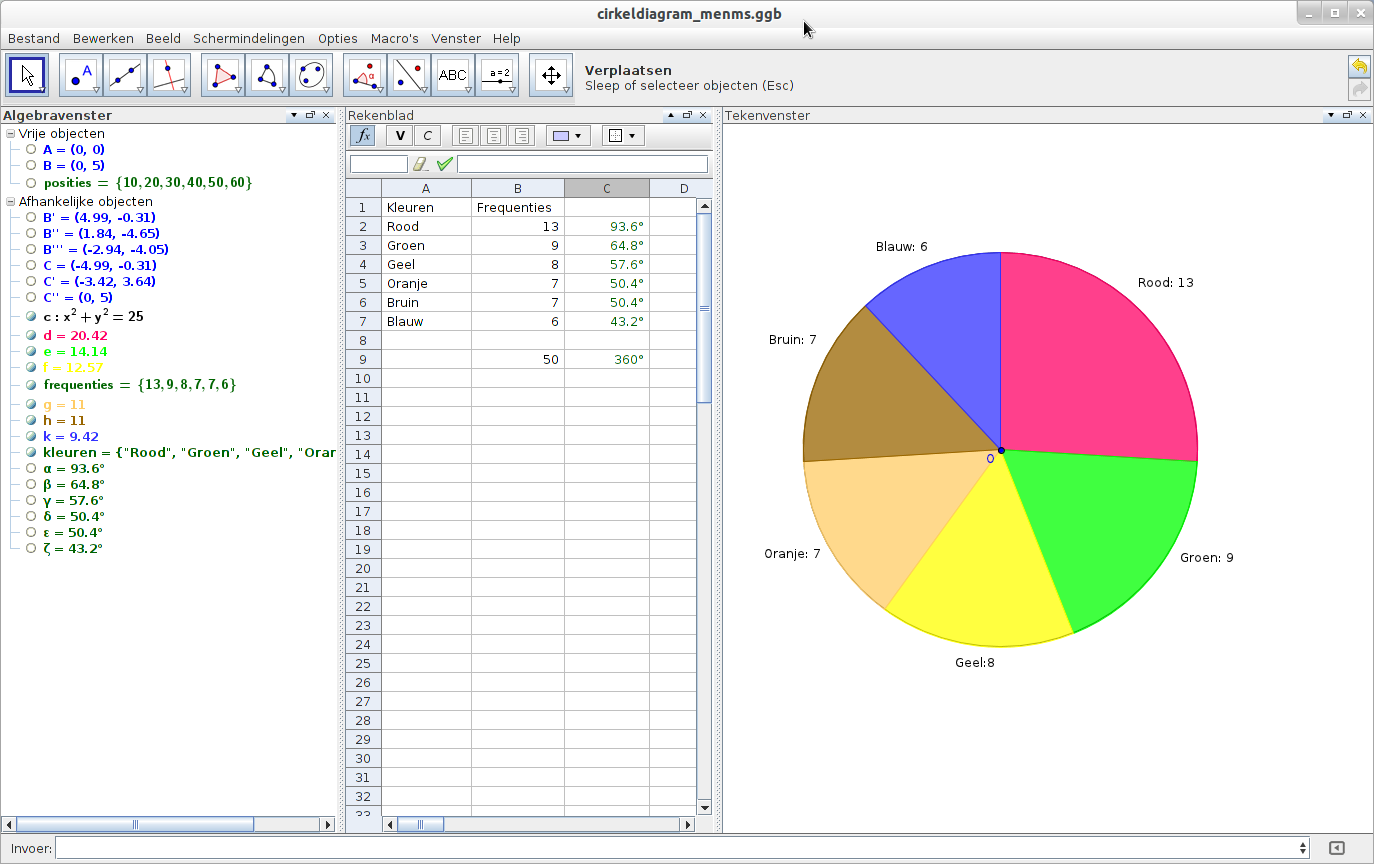
\includegraphics[width=14cm]{gg-cirkeldiagram_menms}
\end{center}

\subsection{Wat heb je gevonden? Hoever kan je gaan in je conclusie?}

\subsubsection{De variabiliteit van steekproefresultaten}

Je hebt nu de kleur van de snoepjes in een zakje M\&M’s bestudeerd met behulp van een
frequentietabel, een staafdiagram en een taartdiagram. Laten we nu eens kijken naar de
inhoud van een aantal andere zakjes M\&M's.

\vraag{Verwacht je dat de andere zakjes dezelfde resultaten zullen hebben als het eerste zakje?}{3cm}

\vraag{Kan je je antwoord op vorige vraag wat verduidelijken door te verwijzen naar de manier
waarop die zakjes gevuld worden? Kan je hierbij ook de woorden populatie en steekproef op
een juiste wijze gebruiken?}{3cm}

In plaats van naar alle kleuren te kijken, zou je er eens je lievelingskleur kunnen uithalen,
bijvoorbeeld blauw. Hoeveel percent blauwe snoepjes zaten er in het eerste zakje? En hoeveel percent
blauwe snoepjes waren er in de andere zakjes?

\vraag{Noteer voor elk onderzocht zakje in je klas telkens het percent blauwe snoepjes.}{5cm}

\vraag{Als jij maar één zakje snoepjes mag onderzoeken (bijvoorbeeld het eerste) en je zou moeten raden hoeveel
percent blauwe snoepjes er door de fabrikant gemaakt wordt (dus hoeveel percent blauwe
snoepjes er in de totale populatie zit), wat zou jij dan antwoorden?}{4cm}

\vraag{Is je bovenstaand antwoord exact juist? Hoe weet je dat?}{3cm}

\subsubsection{Steekproefgrootte, nauwkeurigheid en haalbaarheid}

Met het onderzoek van de snoepjes in een aantal zakjes M\&M’s wil je een zicht krijgen op alle
M\&M-snoepjes. Je zou bijvoorbeeld willen weten hoeveel percent van alle M\&M’s blauw zijn of op
welke manier de kleuren verdeeld zijn.

Een eerste (maar naïeve) reactie zou kunnen zijn: wel, onderzoek dan de totale populatie. Maar dat
voorstel is helemaal niet haalbaar! Je gaat toch niet alle zakjes openmaken om te kijken wat de kleur
van de snoepjes is. Dat zou niet alleen veel te veel tijd en geld vragen, het is gewoon onmogelijk
omdat de snoepjes dan niet meer kunnen verkocht worden. Daarom onderzoek je dus maar een
beperkt aantal snoepjes: je verzamelt informatie over een deel van de M\&M’s om zo conclusies te
trekken over alle M\&M’s.

Herinner je de twee belangrijke begrippen:
\begin{itemize}
  \item De hele groep objecten (of personen) waarover je iets wil weten, heet de {\bf populatie}.
  \item Een {\bf steekproef} is een deel uit deze populatie.
\end{itemize}

Als het praktisch haalbaar is en als je op een goede manier steekproeven trekt, dan is het beter om
met een grotere steekproef te werken dan met een kleinere. Intuïtief kan je dit waarschijnlijk wel
begrijpen. Als je een groter aantal M\&M’s uit de totale populatie mag trekken, dan heb je meer
informatie. Maar ook een grote steekproef is nog altijd aan het toeval onderhevig. Als je echter
meerdere keren een grote steekproef zou trekken, dan zou je zien dat op grotere steekproeven minder
schommelingen zitten dan op kleinere.

Om een grotere steekproef te krijgen brengen we nu alle open gedane zakjes M\&M's samen en gebruiken
we deze als één grote steekproef.

\vraag{De verschillende resultaten van elk onderzocht zakje worden nu verzameld. Noteer alle
cijfers die op bord komen en maak dan een nieuwe frequentietabel met daarin per kleur de
frequentie en de relatieve frequentie voor de snoepjes van de totale klas.}{0cm}

\begin{center}
  \begin{tabular}{|p{2cm}|p{2cm}|p{2cm}|}
    \hline
    Kleur&Frequentie&Relatieve frequentie\\
    \hline
    &&\vspace*{0pt}\\
    \hline
    &&\vspace*{0pt}\\
    \hline
    &&\vspace*{0pt}\\
    \hline
    &&\vspace*{0pt}\\
    \hline
    &&\vspace*{0pt}\\
    \hline
    &&\vspace*{0pt}\\
    \hline
  \end{tabular}
\end{center}
\vspace{1cm}

\subsubsection{Een model voor de populatie}

Hoe de echte populatie van alle M\&M-snoepjes eruitziet, zal niemand ooit weten. Je kan toch niet
naast die productielijn gaan staan en voor die miljoenen (miljarden?) snoepjes de kleur noteren.
Maar een model voor de populatie bestaat wel. In België worden geen M\&M’s gemaakt. Zij worden
ingevoerd uit naburige landen. Bij M\&M’s uit Frankrijk komen alle kleuren globaal (in de populatie)
evenveel voor.

\begin{wrapfigure}[8]{l}{0.3\textwidth}
  \vspace{-0.5cm}
  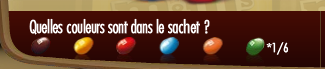
\includegraphics[width=0.3\textwidth]{MenM-uniforme_verdeling}
  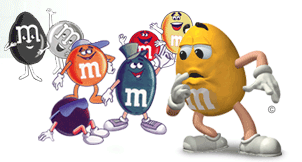
\includegraphics[width=0.3\textwidth]{MenM-hoeveel}
\end{wrapfigure}
Als je nu mag aannemen dat (volgens de fabrikant) alle
kleuren evenveel voorkomen dan kan je deze eigenschap
gebruiken om een model te maken voor de totale
populatie. Aan de andere kant heb jij nu cijfers van een
grote steekproef uit die populatie. Het is dus interessant
om het model voor de populatie te vergelijken met wat je
ziet in die grote steekproef. Je zou hiervoor twee
afzonderlijke staafdiagrammen kunnen tekenen maar je
kan die vergelijking ook in één en dezelfde figuur
voorstellen.

\vraag{Maak een tabel waarin je aangeeft hoe de populatie er precies uitziet. Gebruik je frequenties
of relatieve frequenties in die tabel?}{0cm}

\begin{center}
  \begin{tabular}{|p{2cm}|p{2cm}|}
    \hline
    Kleur&\\
    \hline
    &\vspace*{0pt}\\
    \hline
    &\vspace*{0pt}\\
    \hline
    &\vspace*{0pt}\\
    \hline
    &\vspace*{0pt}\\
    \hline
    &\vspace*{0pt}\\
    \hline
    &\vspace*{0pt}\\
    \hline
  \end{tabular}
\end{center}

\vraag{Hoe ga je de grafiek tekenen? Welke volgorde kies je voor de kleuren op de $x$-as?}{3cm}

\vraag{Teken nu de grafiek.}{0cm}
\begin{center}
  \definecolor{qqqqff}{rgb}{0,0,1}
\begin{tikzpicture}[line cap=round,line join=round,>=triangle 45,x=1.0cm,y=1.0cm]
\draw[-,color=black] (0,0) -- (10,0);
\draw[-,color=black] (0,0) -- (0,10);
\end{tikzpicture}

\end{center}

\vraag{Kan je verklaren waarom jouw cijfers eventueel afwijken van die van de fabrikant?}{3cm}

\subsection{Kernachtige samenvatting van dit onderzoek}

Een statistisch onderzoek wordt niet zomaar in het wilde weg gedaan. Meestal is er een
opdrachtgever (bedrijf, overheid, organisatie, ...) die bepaalde informatie nodig heeft. De statisticus
die het onderzoek heeft uitgevoerd zal dan ook zijn onderzoeksresultaten zorgvuldig moeten
presenteren bij die opdrachtgever.

Op dit ogenblik heb je al heel wat informatie over het onderzoek. Deze informatie moet je nu nog
vervolledigen met:
\begin{itemize}
  \item antwoorden op de contextvragen
  \item besluiten over het uitgevoerde onderzoek.
\end{itemize}

De contextvragen of www-vragen, die bij elk onderzoek aan bod komen, zijn:
\begin{enumerate}
  \item {\bf Waarom} is dit onderzoek uitgevoerd? (Wie wilt wat weten?)
  \item {\bf Waar} is dit onderzoek uitgevoerd? (In het buitenland? In mijn gemeente?)
  \item {\bf Wanneer} is dit onderzoek uitgevoerd? (Vorige eeuw? Dit jaar?)
  \item {\bf Wie of wat} wordt onderzocht? (Bij wie worden dingen opgemeten? Wat zijn de
“elementen”?)
  \item {\bf Wat} wordt er juist opgemeten?( Wat wordt er per element allemaal genoteerd? Wat
zijn de “veranderlijken”?)
  \item {\bf Hoe} wordt dit onderzoek uitgevoerd?( Hoe zijn de “elementen” verzameld? Hoe zijn
mensen bij een enquête gecontacteerd?)
\end{enumerate}

\vraag{Formuleer in een bondige tekst de antwoorden op de contextvragen.}{4cm}

Nu kan je conclusies trekken. Maar je hebt al begrepen dat statistische besluiten rekening moeten
houden met toevallige uitkomsten en dus niet hetzelfde zijn als wiskundige bewijzen.
Wees dus voorzichtig bij je besluit. Als er problemen zijn opgetreden, vermeld die dan. Zo kom je
tot een genuanceerd rapport.

\vraag{Formuleer in een bondige tekst je besluiten over het uitgevoerde onderzoek.}{4cm}

\begin{center}
  
\includegraphics[width=0.3\textwidth]{MenM-snoepjes_banner}
\end{center}

\subsection{Zelfevaluatie}
In dit onderzoek heb je geleerd over:\\
\begin{wrapfigure}[13]{r}{0.2\textwidth}
  \vspace{1cm}
  
\includegraphics[width=0.2\textwidth]{MenM-zelfeval}
\end{wrapfigure}
\vspace{-1cm}
\begin{itemize}
  \item de context van een statistisch onderzoek (wanneer, waar,...)
  \item het onderscheid tussen de populatie en een steekproef
  \item een enkelvoudige aselecte steekproef
  \item de structuur van een dataset (elementen, veranderlijken)
  \item nominaal kwalitatieve veranderlijken
  \item de frequentietabel bij een nominaal kwalitatieve veranderlijke
  \item het staafdiagram bij een nominaal kwalitatieve veranderlijke
  \item het taartdiagram bij een nominaal kwalitatieve veranderlijke
  \item het staafdiagram met subgroepen.
\end{itemize}

Je bent nu in staat om de volgende opdrachten uit te voeren:

\vraag{Zeg in eigen woorden op welke vragen je een antwoord moet kunnen geven als men vraagt
naar de context van een statistisch onderzoek.}{3cm}

\vraag{Omschrijf de begrippen steekproef en populatie in je eigen woorden en geef een (nieuw)
voorbeeld. Leg voor jouw voorbeeld uit hoe je daar een enkelvoudige aselecte steekproef zou
trekken.}{3cm}

\vraag{Leg duidelijk uit hoe een dataset eruitziet. Gebruik hiervoor een nieuw voorbeeld dat je zelf
hebt bedacht.}{3cm}

\vraag{Zeg in eigen woorden wanneer je van een kwalitatieve veranderlijke zegt dat ze nominaal is.
Is de bloedgroep zo’n veranderlijke? Kan je zelf een nominaal kwalitatieve veranderlijke
bedenken?}{3cm}

Als je opmetingen hebt van een nominaal kwalitatieve veranderlijke, dan moet je daarvoor
een frequentietabel, een staafdiagram en een taartdiagram kunnen maken

Soms kom je de uitdrukking “horizontaal staafdiagram” tegen. Kijk daarvoor naar de figuur
die je vindt in de Gazet van Antwerpen van 3 november 2004. Voor de 364 jobs die in
oktober 2004 bij de 4 grootste faillissementen in Vlaanderen verloren gingen, heeft men een
figuur getekend.

\begin{center}
  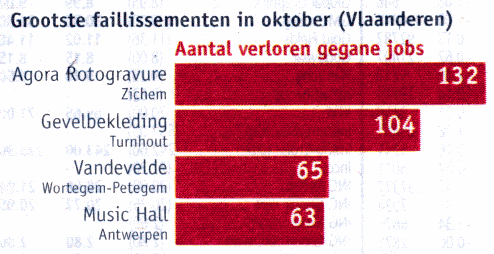
\includegraphics[width=0.6\textwidth]{horizontaal_staafdiagram-faillissementen}
\end{center}

\vraag{Welke veranderlijke is er genoteerd bij elke persoon die zijn job is
kwijtgeraakt? Welk soort veranderlijke is dat? Wat zijn haar waarden? Is de figuur goed
getekend?}{4cm}

\newpage

\begin{wrapfigure}[6]{r}{0.4\textwidth}
  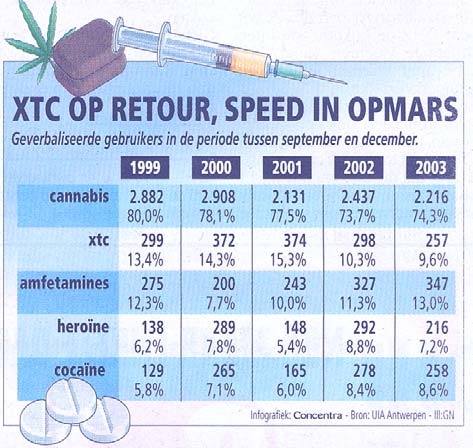
\includegraphics[width=0.4\textwidth]{tabel-drugs}
\end{wrapfigure}

Als je een frequentietabel ziet, dan moet je
die juist kunnen interpreteren. Bekijk de
tabel over XTC en Speed (Gazet van
Antwerpen van 20-10-2004). Kijk enkel
naar de informatie die daarin staat over het
jaar 2003.

\vraag{Is “druggebruik” daar
behandeld als een nominaal kwalitatieve
veranderlijke? Is de tabel correct?}{4cm}

Een bestaande figuur moet je juist kunnen interpreteren. Bekijk het taartdiagram over de
vrijetijdsbesteding van jongeren (De Standaard van 6-12-2000).

\begin{center}
  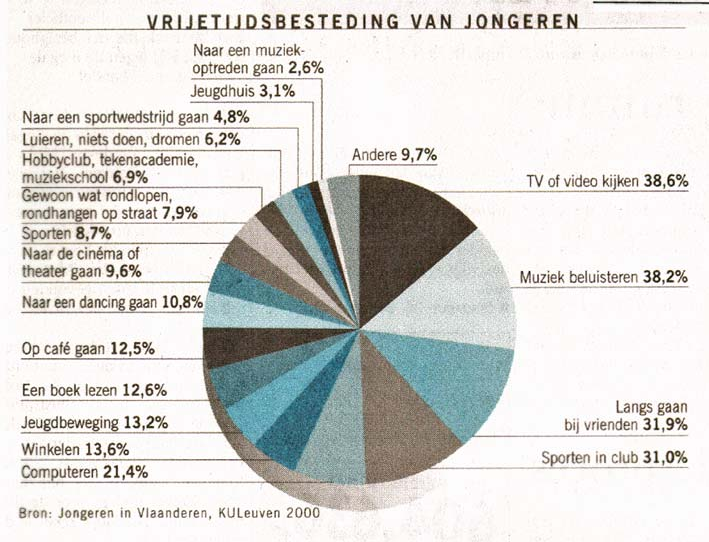
\includegraphics[width=0.6\textwidth]{cirkeldiagram-vrijetijdsbesteding}
\end{center}

\vraag{Is “vrijetijdsbesteding” hier behandeld als een nominaal kwalitatieve veranderlijke? Is het taartdiagram correct getekend?}{4cm}

\section{Een statistisch onderzoek naar het schatten van de tijdsduur van 1 minuut}

\subsection{Wat wil je weten? Hoe ga je meten?}

\subsubsection{De onderzoeksvraag}

In sporten zoals atletiek, zwemmen, Formule 1, speelt tijdsopname een belangrijke rol. Probeer je
eens voor te stellen wat in de cockpit van een Ferrari gebeurt om de rondetijden tot op een duizendste
van een seconde te kunnen opmeten.

De meest primitieve manier van tijdsopname is vermoedelijk gewoonweg ... tellen. Je kent
waarschijnlijk het 21 – 22 – 23 trucje om 3 seconden te benaderen, maar de tijdsduur van één minuut
schatten is heel wat moeilijker. Of niet? Aan jou de uitdaging om dit te onderzoeken!

Let op! Wat is je populatie?\\
Je hebt hier opnieuw een probleem. Je moet eerst heel nauwkeurig zeggen wat je bij welke populatie
wil onderzoeken. Misschien wil je weten hoe één bepaalde leerling een minuut schat, om te
constateren dat zij een kwart van de keren te hoog en drie kwart van de keren te laag schat. Dan
bestaat je populatie (in theorie) uit alle resultaten van die leerling, als je die miljoenen keren een
minuut zou laten schatten. En als steekproef zal je dan die éne leerling 40
keren laten schatten. Zo krijg je een idee over het schattingsgedrag van die
éne leerling.


\end{document}


\begin{wrapfigure}[13]{r}{0.3\textwidth}
  \includegraphics[width=0.3\textwidth]{figuur}
\end{wrapfigure}






















